\section{Copyright Notice \& License}

    Copyright (C)  2024 Leandro Ebner. \\
    Permission is granted to copy, distribute and/or modify this document under the terms of the GNU Free Documentation License, Version 1.3 or any later version published by the Free Software Foundation; with no Invariant Sections, no Front-Cover Texts, and no Back-Cover Texts. A copy of the license can be found here:
    \href{https://www.gnu.org/licenses/fdl-1.3.txt}{https://www.gnu.org/licenses/fdl-1.3.txt}.

    \begin{figure}[h!] %Float specifier check: passed!
        
\includegraphics{contents/figures/gfdl-logo.png}
        \hspace{5mm} %HORIZONTAL SPACE
        
\includegraphics[width=1.5cm]{contents/figures/DOI_logo.png}
        \href{http://dx.doi.org/10.13140/RG.2.2.30250.22723}{10.13140/RG.2.2.30250.22723}
    \end{figure}

    \vspace{5mm} %VERTICAL SPACE
    
    This document is built using several packages originally developed by Stefan Gast for being compliant with RWU's corporate design. Due to the fact that repository is archived now, an active fork is available for public at: \\
    \href{https://github.com/leandroebner/latex-rwustyle}{https://github.com/leandroebner/latex-rwustyle} 

    The source code to build this document, including all relevant information about the R2M project is available in a dedicated GitHub organization and actively maintained by its contributors: \\
    \href{https://github.com/RWU-R2M}{https://github.com/RWU-R2M}
    
\section{Introduction}

    This document will serve as a comprehensive guide through the entire power distribution and wiring system of the rover. It meticulously details all relevant safety measures designed to minimize the likelihood of hazards or environmental damage. By following these guidelines, we aim to ensure that our work adheres to the highest safety standards. In addition to outlining essential safety protocols, this guide sets forth the minimum standards for both material and personal safety. These standards apply not only during the construction phase but also throughout the actual operation of all electronic components during the competition. To enhance understanding and clarity, it includes several schematics, data sheets, and detailed calculations. These resources are designed to provide a thorough illustration of the rover's internal architecture and functionality, making the document as informative and accessible as possible.

    \begin{table}[b!] %Float specifier check: passed!
        \centering
        \begin{tabular}{|r|r|r|r|} \hline %MUST REMAIN "R" TO BE COMPLIANT WITH INITAL RELEASE ON GITHUB. DO NOT CHANGE!!
             Revision& Date submitted& Summary of changes&  Authored      \\ \hline 
             v1.1.0&   23.06.2024&     1st CSTAG evalution& Leandro Ebner \\ \hline 
             v1.0.0&   16.06.2024&     Initial release&     Leandro Ebner \\ \hline
        \end{tabular}
    \end{table}

    \clearpage %PAGE SPECIFIER
    
\section{Hazardous Materials}

    \subsection{Batteries}
    
    The rover is using two lithium-polymer based batteries (further referred to as LiPo batteries) to power all the electronics. Batteries, in general, are compliant with the regulations set by the CIRC (see \ref{battery} of the appendix) as long as they are sealed and follow certain safety guidelines (i.e. using battery-management-systems to ensure usage within manufacturer-specifications). LiPo batteries are designed as permanently sealed units, which contain their electrolytes within durable casing materials. This prevents the escape of hazardous substances under normal operating conditions. This cell chemistry is widely used in consumer electronics, remote-controlled vehicles, and other devices where safety and environmental compliance are critical and high electrical characteristics are required. This demonstrates their reliability and safety under proper use and are known for a high energy density as well as output power capability. For this reason, the LiPo cell chemistry was also utilized for energy storage in the rover.
    
    \vspace{5mm} %VERTICAL SPACE
    
    LiPo batteries feature a nominal voltage of around $3.7V$ per cell, depending on the exact type of internal chemistry. Higher output voltages are achieved by connecting several individual cells in series with each other, still being housed in the same battery enclosure. Therefore, the (series) cell count of a LiPo battery is a fundamental property of any LiPo battery and a direct measure for the expected output voltage. Usually, this property is indicated in the following way: "3S LiPo Battery", whereas "3S" is referring to a total series cell count of three. This results in a nominal voltage of around $11.1V$. For this exact reason, LiPo batteries can't be manufactured for an arbitrary output voltage and certain compromises must be made. The rover is built upon the idea of having a $24V$ battery supply as the main voltage for high power applications and another $12V$ battery supply for all logic and controlling components. This results in a 6S and 3S configuration of battery cells to closely match those voltages. Those common naming conventions must be known to safely work with batteries, including charging/discharging them in a safe manner. Detailed information about the two batteries used in the rover can be found in their datasheet \ref{prim-battery} and \ref{sec-battery} respectively. The concept of using multiple batteries during normal operation in the rover compared to single power source will be further addressed.

    \clearpage %PAGE SPECIFIER   
    
\section{Power Design Illustration}

    The rover's power architecture is divided into two separate power systems. This approach ensures galvanic isolation between the power and logic components, which is necessary to eliminate any possible wiring configuration in which a so-called "ground loop" could form. The underlying problem is based on the fact that there exists an interface and thus an electrical connection between the individual components. While the communication between power and logic components is implemented by establishing a physical connection between their corresponding GPIO pins and reading different voltage levels, there must be a precise reference voltage available at any given point in time. Generally speaking, this is done by using a common ground. Hence, the most basic form to utilize that common ground connection is to form a "star ground." If there are multiple paths to ground, a ground loop is present. These ground loops, in combination with wire inductance, can cause issues for high-current electronics like the rover's motor controllers (in this particular case utilizing "ODrives"). This is further illustrated in figure \ref{ground_loop_bad}.
    
    \begin{figure}[h] %Float specifier check: passed!
        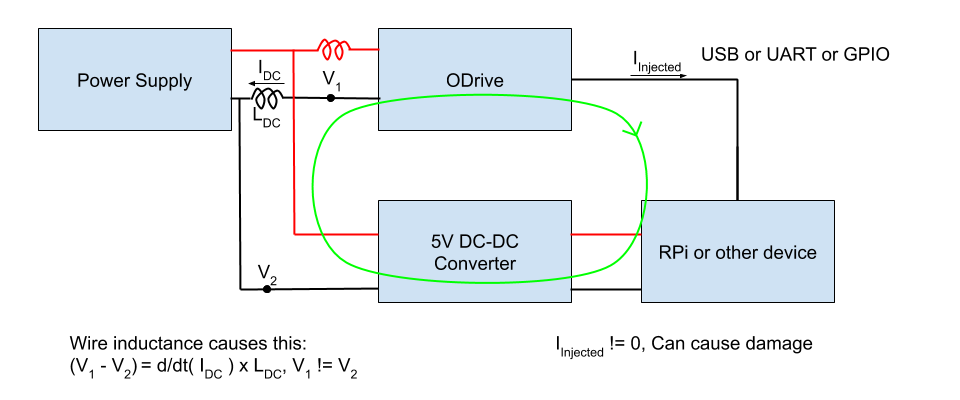
\includegraphics[width=\textwidth]{contents/figures/ground_loop_bad.png}
        \caption{Ground loop causes current flow $I_{Injected}$.}
        \label{ground_loop_bad}
    \end{figure}
    
    The issue is the inductance of the power wires between the motor controllers and the battery. This inductance, coupled with the high current drawn by the motor controllers, causes $V_1$ to be different as $V_2$, leading to potential mismatch in the voltage levels. As the motor controllers demand substantial current, the wire inductance can generate significant voltage drops along the power lines. If the voltage caused by the wire inductance and current is high enough, the $0-5V$ GPIO signals can swing much higher or lower than the defined voltage range, potentially exceeding safe operational limits. These fluctuations in voltage can introduce erratic behavior in the control system, compromising the performance and reliability of the motor controllers. This causes a current to flow through the ODrives's GPIO pins, which can lead to unintended electrical noise and potential damage to sensitive electronic components.

    \clearpage %PAGE SPECIFIER
    
    \subsection{Reducing length of high-current wires}
    
    To mitigate these effects, it is substantial to keep the main power wires as short as possible. All wires have some amount of inductance, which is an inherent property of any conductor through which current flows. The inductance is proportional to the length of the wires and the area of the loop formed by the power wires, meaning longer wires and larger loops will have higher inductance. This inductance can create unwanted resistance to changes in current flow, leading to voltage drops and potential interference with the system's performance. It is beneficial to keep those wires as short as possible and as close together as possible. By doing so, the loop area is minimized and the inductance is reduced, thereby mitigating the adverse effects. However, this reduces the effect of the problem but does not eliminate it entirely, as even minimal inductance can cause issues in high-frequency and high-current applications.
    
    \subsection{Galvanic isolation}
    
    To completely minimize the possibility of creating ground loops by accident, the loop must be broken. This can be achieved by isolating the power supplies (no common ground) and connecting a dedicated signal ground between the logic and power electronics. An example of this is a single motor controller connected to a battery and a device like a Raspberry Pi connected to a different battery. It is possible to achieve the same functionality with a DC/DC isolator as shown in figure \ref{ground_loop_fix}. By isolating the data connection (whether it is GPIO, USB, or UART, etc.), the ground loop is broken.
    
    \begin{figure}[h] %Float specifier check: passed!
        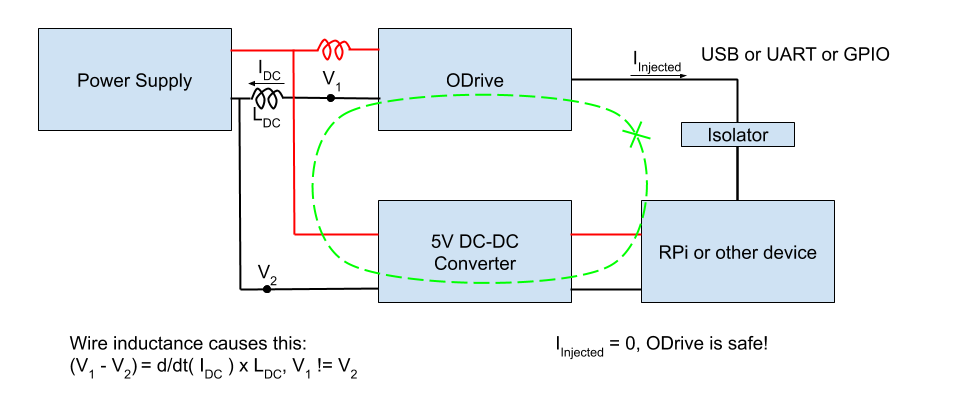
\includegraphics[width=\textwidth]{contents/figures/ground_loop_fix.png}
        \caption{Mismatched voltage levels wont introduce unwanted current flows.}
        \label{ground_loop_fix}
    \end{figure}

    \clearpage %PAGE SPECIFIER
    
\section{Basic Electric Layout}

    While it would be possible to use DC/DC isolators whenever a ground loop could appear, it is more straight forward and easier to implement a complete different power solution. The main energy storage contains the unregulated $24V$ (6S) and $12V$ (3S) power sources in the form of LiPo batteries. This part of the rover also integrates a dedicated battery management system (further referred to as BMS) for each battery. Additionally, the main fusing for the primary \& secondary battery can be found here. The fuses protect the rover's circuitry as well as the batteries themselves. Due to the fact, that these components are strictly connected to the individual batteries, they change frequently with each battery exchange during normal operation. This means that during missions, the batteries can be quickly replaced without affecting other parts of the rover. Therefore, this area is separated from other areas of the rover's wiring as it is the only region where connections and disconnections of components are allowed. This separation is crucial to avoid accidental disconnections that could affect the rover's operation or create potential risks by introducing faulty connections. The output of both batteries is directly fed into an emergency stop system. Afterwards, the power travels into two separate distribution and fusing circuits before supplying the actual components and voltage converters further down the line. To illustrate that, see the attached figure \ref{power_architecture}.
    
    \begin{figure}[h] %Float specifier check: passed!
        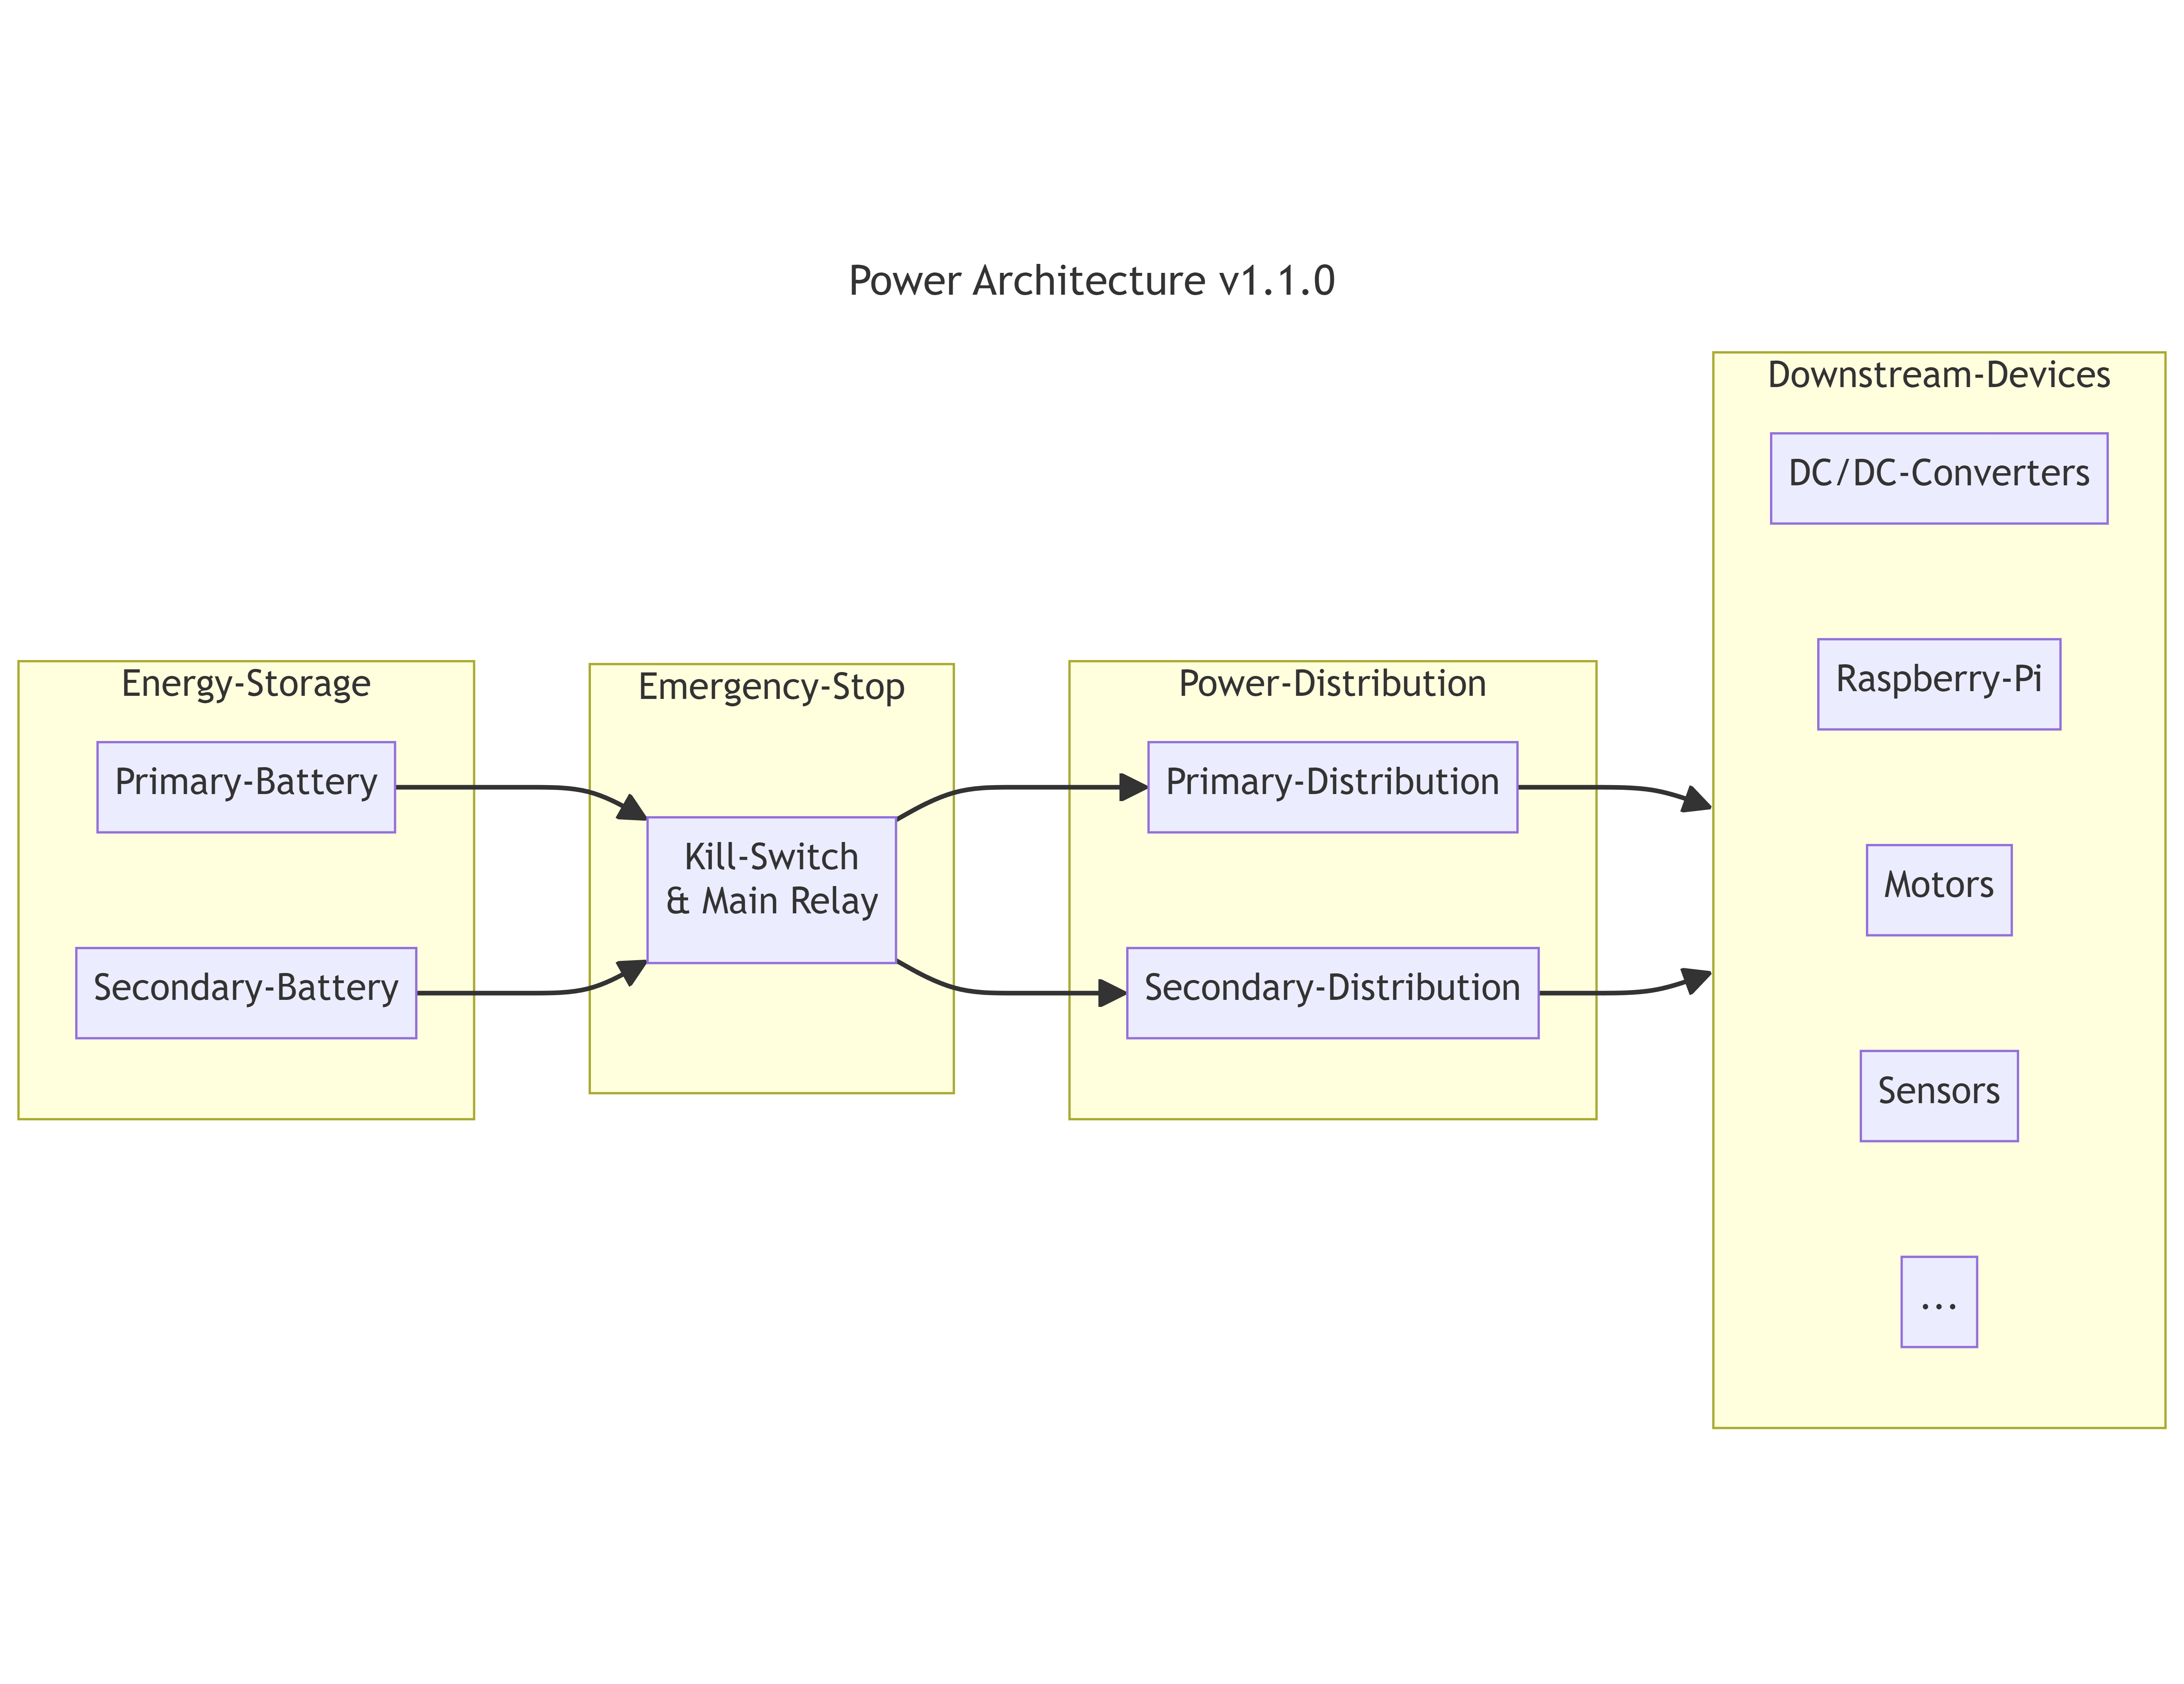
\includegraphics[width=\textwidth]{contents/figures/power-architecture-v1.1.0.png}
        \caption{Basic electrical layout split in the main 4 categories. Each category serves a different purpose (in example safely distributing the power or connecting the individual components with each other).}
         \label{power_architecture}
    \end{figure}

    \clearpage %PAGE SPECIFIER

    \subsection{Voltage rails}

    The rover provides 4 different main voltage levels to the individual components. The primary and secondary LiPo batteries output the unregulated $24V$ and $12V$ power. This choice is based on the fact that those two voltages are quite common in the industry and are used in various fields of applications. As already mentioned, the $24V$ power rail is paired with all the devices demanding high power and therefore coming with a high current draw. Big currents always go hand in hand with the necessity of larger wire cross-sections, which results in increased costs, weight and more challenging wiring. This is a direct cause of "Ohm's Law". The total electrical power P is defined as $P_{Electrical}=U*I$. Using a higher voltage can help to tackle those problems due to lowering the overall current-flow, while also improving the total efficiency of the system as a side effect. Less power being dissipated in the form of heat is one cause of that, which can be calculated as $P_{Loss}=R*I^2$ . The best-case scenario would be close to no voltage regulating components at all, powering everything directly by the voltage the batteries supply on their own. This is however not always possible. Using a standardized supply voltage to determine what battery to use is a good approach to minimize the need of voltage converters and to keep the complexity low. While there exist components and systems for higher voltages like $48V$, they come with a significantly bigger problem when used in combination with battery power. The output power of a battery does not remain constant during a normal charge/discharge cycle. During normal operation, the voltage of each battery cell fluctuates at around $0.8V$. Pairing more battery cells in series also increases the absolute voltage difference between a fully charged and discharged battery. While components with internal voltage regulators may handle that without noticeable difference, others may be become unstable or get overloaded by the supply, depending on the remaining charge of the battery. Keeping the primary battery voltage at $24V$ is a good compromise between power efficiency and absolute voltage stability. Additional voltage-converters are introduced in the relevant upcoming chapters.

    \vspace{5mm} %VERTICAL SPACE

    Due to the fact the unregulated $12V$ rail is only used and intended for low-energy appliances to minimize complexity and load of the battery and secondary circuit, $12V$ is sufficient in this case. Also, this doubles as second native voltage source besides the primary supply. There is also a dedicated buck-converter for having a high power $12V$ rail to step down the $24V$ of the primary battery. That converter is used in combination with the servo-motors for steering the rover. This step was mandatory, because the servo-motors are not connected to another motor driver or similar circuit and are run directly by the voltage applied to their terminals. That will ensure a stable applied voltage and keeps a margin of flexibility of what type of servo-motors to use. 

    \clearpage %PAGE SPECIFIER

    \subsection{Wire cross-sections}

    All the wires can be classified into four different groups. There is one type of wire only used for carrying signals, thus having the smallest cross-section of all of them. For power-carrying wires, you can sort them into three different groups, reaching from low, medium to high current wires. According to the table \ref{color_codes}, they are $1.5mm^2$, $4.0mm^2$ and $10.0mm^2$ in area. As one might expect, all cables can come in various colors and there is no fixed internal guideline what those colors may represent. The rover's wiring sticks to common conventions for marking positive, negative and auxiliary wires in descrete colors always. To easily tell and differentiate the cross-sections of arbitrary cables, a predefined color-code for each wire type has been set. Those are oriented in respect to the new "DIN 46228" by also making use of the normed abbreviations of the "IEC 60757" standard. White coding marks signal wires, black coding low power wires, grey and red codes are reserved for medium and high current wires. The ampacity per wire also documented in table \ref{color_codes} below.
    
    \begin{table}[h] %Float specifier check: passed! 
        \centering
        \begin{tabular}{|r|r|r|r|r|} \hline 
          color\footnotemark[1]&  code\footnotemark[2] \& HEX format&  cross-section\footnotemark[3]&  equivalent to&  ampacity\footnotemark[4] \\ \hline 
                          white&          WH \#FFFFFF&                    $0.5mm^2$&                          21 AWG&                 7 Amps    \\ \hline 
                          black&          BK \#000000&                    $1.5mm^2$&                          16 AWG&                18 Amps    \\ \hline 
                           grey&          GY \#808080&                    $4.0mm^2$&                          12 AWG&                30 Amps    \\ \hline 
                            red&          RD \#FF0000&                   $10.0mm^2$&                           8 AWG&                55 Amps    \\ \hline
        \end{tabular}
        \caption{Internal R2M guideline defines a fixed set of wires to choose from. The outline ensures consistency and reduces overall complexity. Optionally, those connections can be furthermore labeled with text and color.}
        \label{color_codes}
    \end{table}

    Instead of using a generic ampacity-table in the same fashion CSTAG provided an \href{https://web.archive.org/web/20230310184047/https://www.coonerwire.com/amp-chart/}{\textbf{\underline{example}}}, the current-values have been calculated for the case of 2 or 3 conductors together in a raceway, conduit, or common cable. The given example was refering to a single conductor in free air. This scenario is much less realistic in real-life applications while also providing less headroom if the wiring is done differently. The ampacity in table \ref{color_codes} holds true for an insulation temperature up to 90°C in respect to an ambient temperature of 30°C. The ambient temperature in Drumheller in summer is close to 40°C, and needs to be accounted. This correction should also address the fact that the temperature inside the rover is likely 20°C higher than outdoors, depending on cooling strategies, rover material, paint colour, and other factors. For a total ambient temperature rise up to $\Delta T_{max} = 30K$, a factor as low as $\lambda = 0.71$ as stated in the "NFPA 70" can be applied. Those steps ensure compliance with the CIRC regulation \ref{nfpa}.

    \footnotetext[1]{Ferrule colors according to \textbf{DIN 46228}}
    \footnotetext[2]{Color abbreviations according to \textbf{IEC 60757}}
    \footnotetext[3]{Cross-section according to \textbf{IEC 60228}}
    \footnotetext[4]{Ampacity according to \textbf{NFPA 70, Table 310.15(B)(16)}}

    \clearpage %PAGE SPECIFIER

    \subsection{Power connectors \& wire terminations}

    For terminating the wires, either wire ferrules or nylon (polyamide) connectors have been used. Only "DIN 46228" compliant wire ferrules are used in the rover, sticking to our already existing color scheme. Also, by following the DIN norm, the ferrules will always be suited for the current related to the cross section they are terminating. Similar to the set of wires and wire ferrules, power connectors have been chosen beforehand to follow the electrical requirements. There is a selection of three nylon (polyamide) based connectors named "XT30" (see \ref{xt30}), "XT60" (see \ref{xt60}) and "XT90" (see \ref{xt90}). Their current rating in the same order reaches from $15A$, $30A$ to $40A$. The rating of the connector naming scheme refers to an approved short burst current up to twice of their constant current rating. Also, all power-delivering connectors are highly temperature resistant. As a critical point of failure, where contact resistances have a big influence, this is a precautions step, mandatory for dealing with high currents where short-circuits very likely introduce fire hazards. The fire resistance has been tested according to "IEC 60695-11-10" and all connectors passed the result "94V-0". Further information can be extracted in the appendix.

\section{Dispatch About Creating Diagrams}

    The exact wiring of the rover may vary at any given point in time, especially during the high development phase in the beginning of the electrical construction. To keep track of those physical snapshots and to make updating the documentation easier in the long-term run, a versioning system has been implemented. It's built upon the idea of "Semantic Versioning", a specification originally authored by \href{https://tom.preston-werner.com/}{\textbf{\underline{Tom Preston-Werner}}}. This allows to easily change things in the future by incrementing either the major/minor or patch version of the diagram release. By using the program "Git" to manage and "GitHub" to host those releases, old revisions of diagrams will be archived and the changes between each revision remains accessible anytime. To furthermore benefit from the broad functionality of Git, diagrams are not directly created with the help of an ordinary "WYSIWYG" editor, instead they are written in a markup language (= "WYSIWYM" in this case) and rendered into a separate graphic later. 

    \vspace{5mm} %VERTICAL SPACE

    All diagrams are written with the help of the JavaScript-based tool "Mermaid". Diagrams and documentation itself cost precious time to come up with and suffer from being outdated fairly quickly, as long as the development continues. Those issues can be managed by taking advantage of JavaScript-based graphics and diagrams. The R2M documentations can catch up with development while appearance and format of every diagram can be altered later on, focusing on the actual content first. This is especially useful to follow the CIRC requirement \ref{req7.5} to guarantee the diagrams reflect ongoing changes.

    \clearpage %PAGE SPECIFIER

\section{Wiring Diagram}

    The top level architecture of the rover can be found on the next pages (figure \ref{wiring_diagram}). For clarity, details such as connector types and current return cables have been omitted and will be shown in the smaller fractions further on within this document. As already mentioned, the diagrams group several parts into discrete blocks/areas, to make it look more structured at a glance. Compared to the power architecture (see figure \ref{power_architecture}), which is just a general way of showing the composition of electronics, the wiring diagram (table \ref{wiring_diagram_legend}) provides information about the voltage supplied by the wire (and differentiates between regulated and unregulated supplies), the cross section it has and for what connection it is set-in. 

    \vspace{5mm} %VERTICAL SPACE
    
    \begin{table}[h]
        \centering
        \begin{tabular}{|r|r|l|} \hline 
             color&   code\footnotemark[1]&         voltage specifications\\ \hline 
             red&     RD&                           $22.2V_{nominal}$ (6S Batt -> $24V$ unregulated)\\ \hline 
             orange&  OG&                           $11.1V_{nominal}$ (3S Batt -> $12V$ unregulated)\\ \hline 
             green&   GN&                           $12V_{stable}$ ($V_{in}=V_{Prim-Battery}$, $P_{out}=120W$)\\ \hline 
             blue&    BU&                           $5V_{stable}$ ($V_{in}=V_{Sec-Battery}$, $P_{out}=60W$)\\ \hline 
             black&   BK&                           $3\phi$ AC for Drivetrain ($V_p \approx V_{Prim-Battery}$)
         \\ \hline\end{tabular}
        \caption{To avoid confusion, a distinction between voltage-levels must be made, especially to emphasize the difference between regulated and unregulated supply voltages. }
        \label{wiring_diagram_legend}
    \end{table}

    \footnotetext[1]{Color abbreviations according to \textbf{IEC 60757}}

    \vspace{5mm} %VERTICAL SPACE

    \subsection{Fusing}
    
    Fuses are crucial in electronics, including rovers. Automotive fuses are especially suitable for this purpose, as they are designed to protect vehicle wiring and electrical equipment, typically rated for circuits up to 32 volts DC. They are also commonly used in other low voltage DC systems, such as those in towed campers and marine applications like sailboats and smaller motorboats. To maintain simplicity, the rover uses a single size of automotive fuse known as the "ATO" type, standardized under ISO 8820-3. The broad availability and wide variety of current ratings make these fuses are appropriate choice while keeping the costs low reasonable having several circuits that need to be protected.

    \vspace{5mm} %VERTICAL SPACE

    To eliminate time consuming replacements and also speed up debugging scenarios, thermal circuit breakers in the formfactor of ATO fuses are used. When the circuit breaker trips, the integrated switch function enables immediate reactivation. Unlike a fuse, the circuit breaker does not need to be replaced. 

    \clearpage %PAGE SPECIFIER
    
    Similar to convectional fuses, they come with a distinct trip-behavior: The higher the overload, the faster the thermal circuit breaker trips. This is depended of the absolute current rating and the fuse's specified characteristic. All fuses built into the rover use a uniformly internal naming scheme with the following pattern: "\$A \$-Fused". 

    \vspace{5mm} %VERTICAL SPACE
    
    \begin{wrapfigure}{r!}{0.6\textwidth} %this figure will be at the right
        \centering
        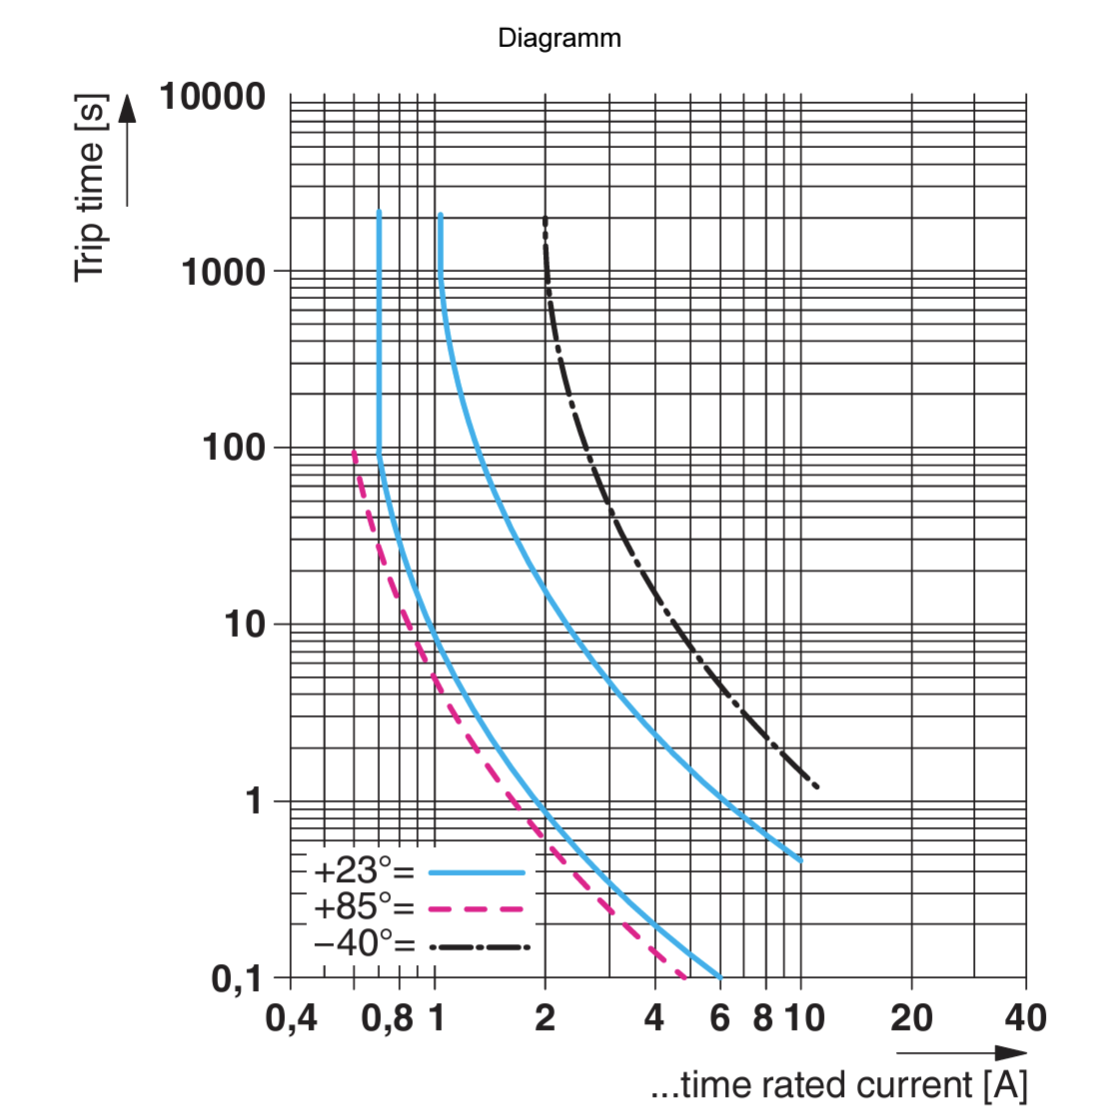
\includegraphics[width=0.6\textwidth]{contents/figures/f-type-fuse.png}
        \caption{TCP with fast trip-response.}
        \label{f-type}
        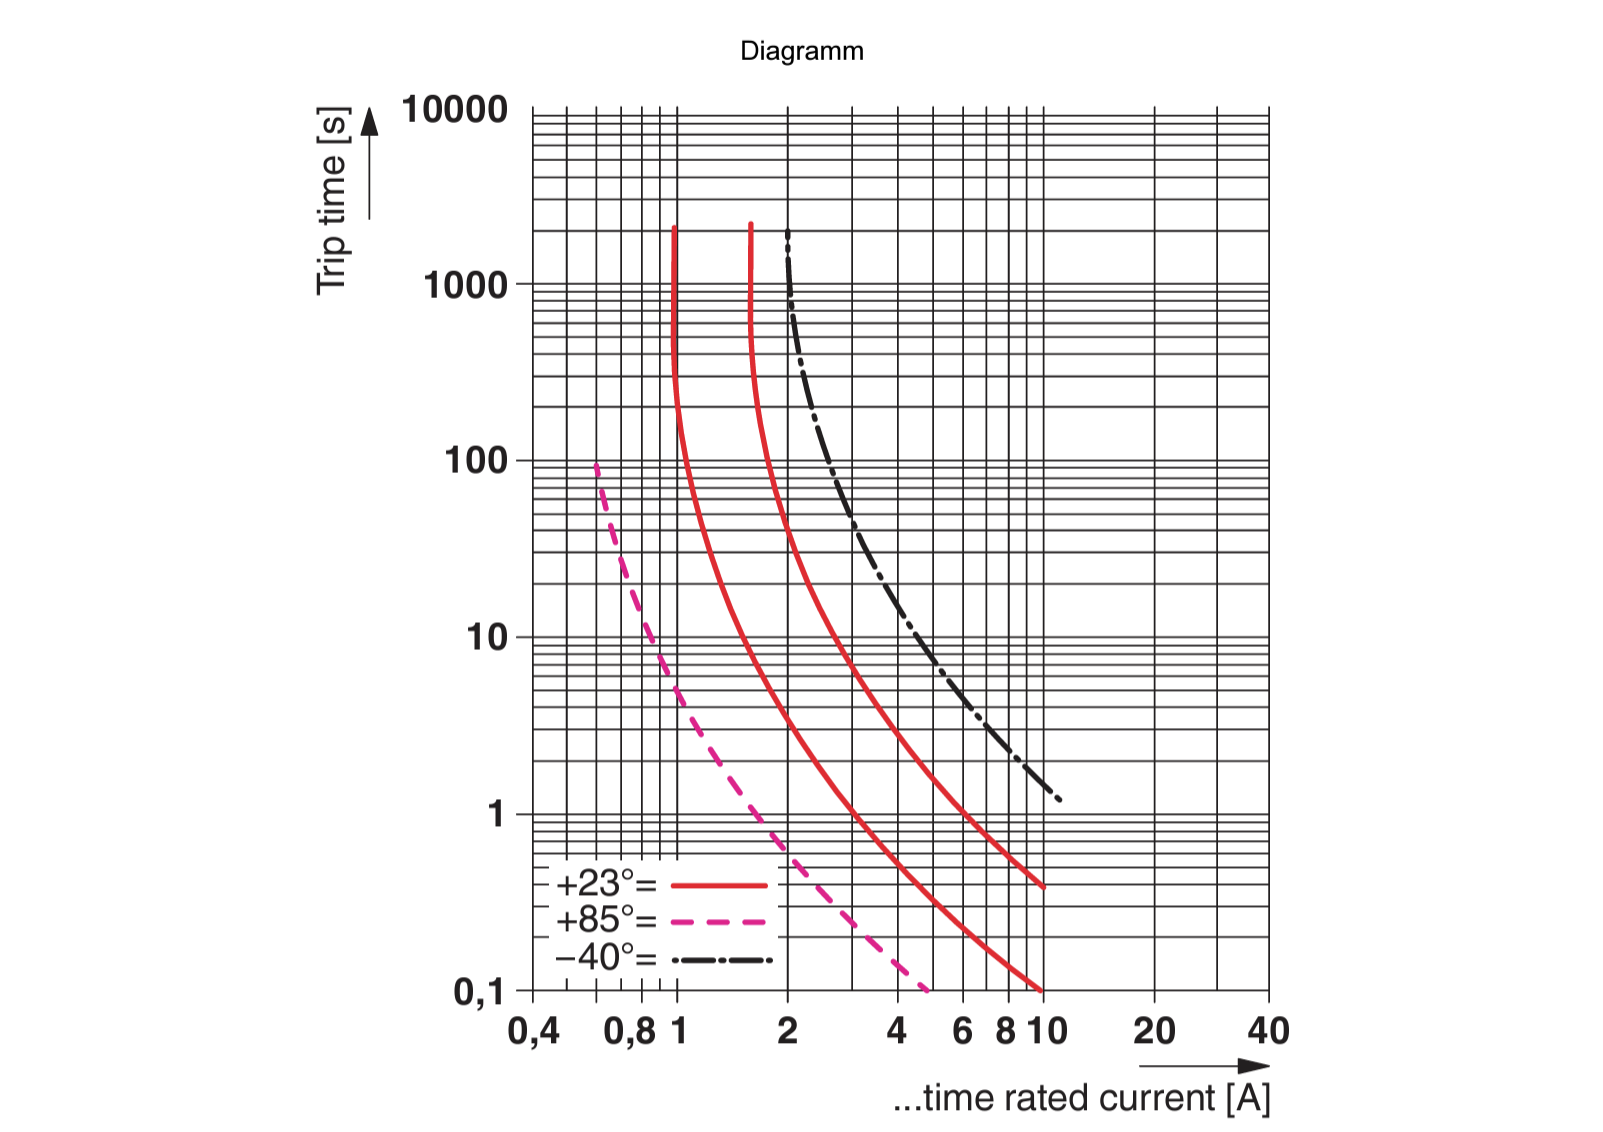
\includegraphics[width=0.6\textwidth]{contents/figures/m-type-fuse.png}
        \caption{TCP with medium trip-response.}
        \label{m-type}
    \end{wrapfigure}

    In this naming convention, the current rating and trip-behaviour is given as a variable. The special thermal-triggered fuses will be refereed to as "TCP" (= Thermal Circuit Protection). There are 2 different trip-response-characteristics for TCPs supplied by "Phoenix Contact", being fast and medium fast. The diagrams for their response can be seen in figure \ref{f-type} as well as in figure \ref{m-type}. In general, "M-type" fuses were used where a wider variation of current draw can occur. This is the case for the drive train or other components directly powered by the battery (high inrush current). For components using a DC/DC converter, the upstream fuse is following "F-type" trip-responses. The reason behind this is, that DC/DC converters usually come with onboard e-fuses and cap out at distinct ampacitys. If the current is higher than specified in the datasheet of the converter, the fuse needs to switch off immediately. 

    \clearpage %PAGE SPECIFIER

    \begin{figure}[ht!] %Float specifier check: passed!
        \paragraph{Top Level Architecture:}
        \centering
        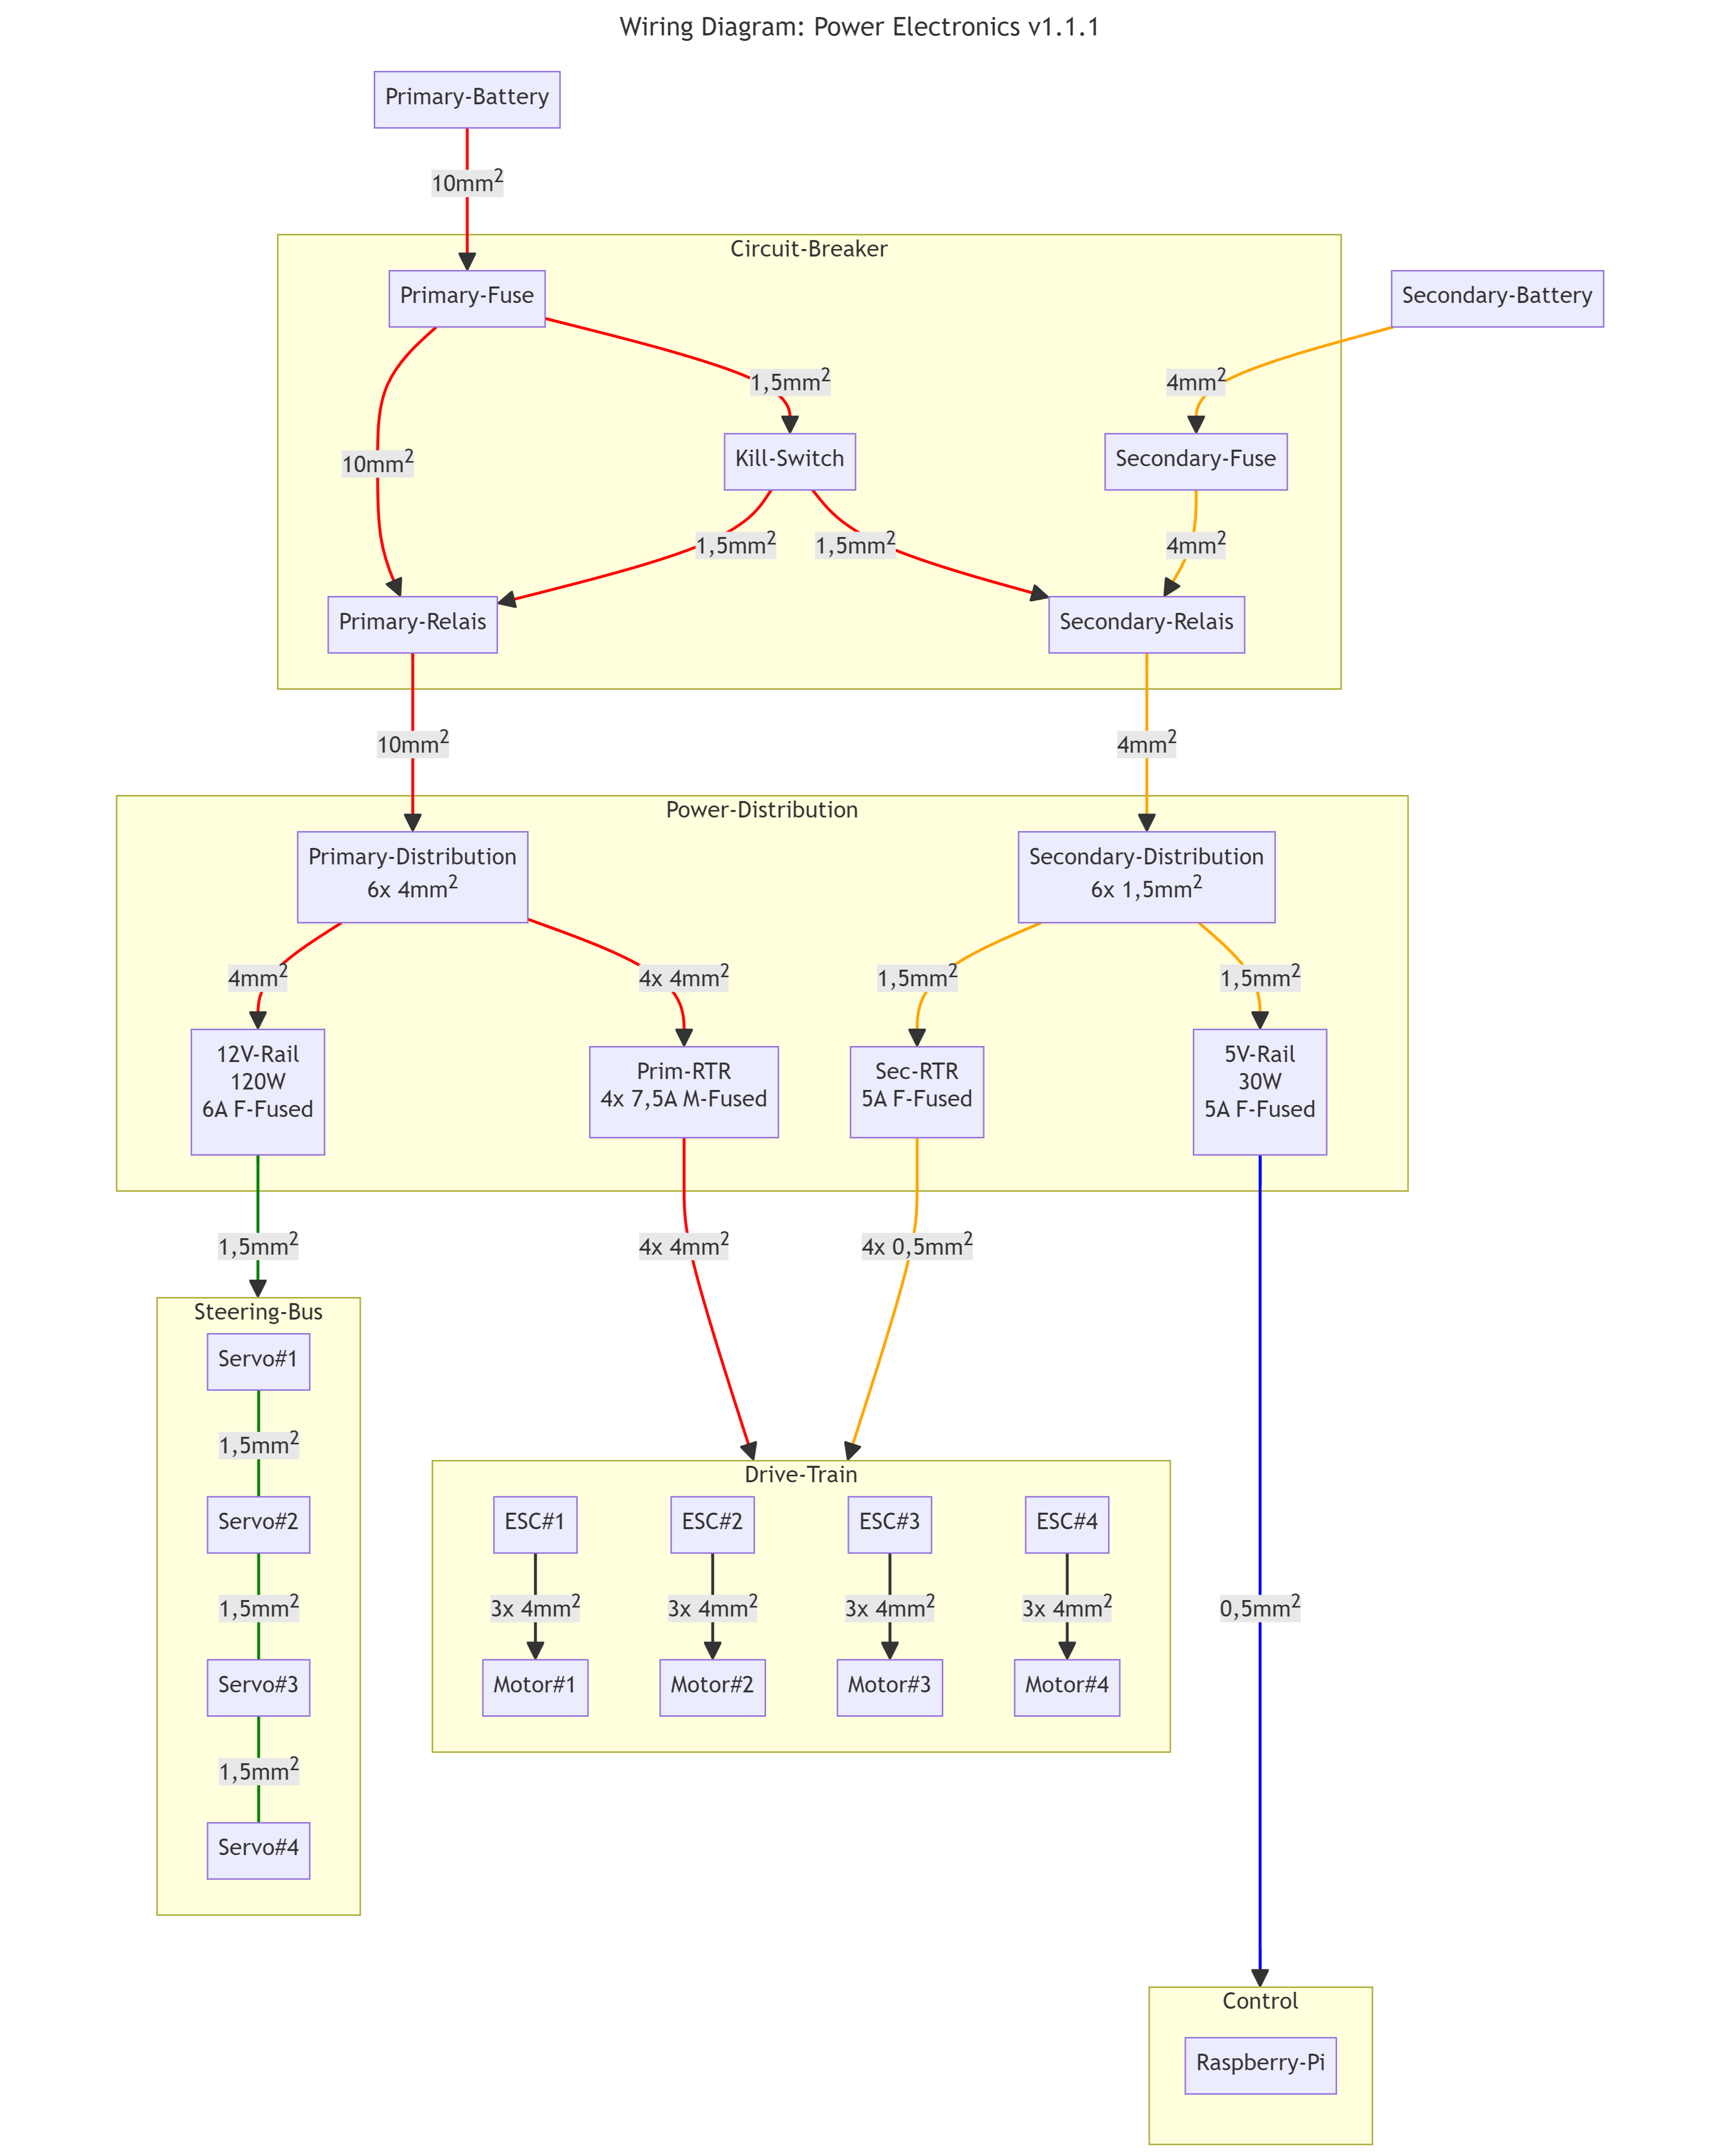
\includegraphics[width=1\textwidth]{contents/figures/wiring-diagram-p-v1.1.1.png}
        \caption{The wiring diagram incorporates several different aspects about how the rover is wired up, including the individual wire cross-sections, voltages and physical location of connections.}
        \label{wiring_diagram}
    \end{figure}

    \clearpage %PAGE SPECIFIER

    \subsection{CAD planning of DIN-mounting-rails}

    Sticking to industrial standardized mounting rails for the main wiring and distribution box is favourable. To accomplish this process, blueprints in CAD have been created to fit all the components and distribution blocks inside of a custom built wiring enclosure/switching cabinet later on. 

    \begin{figure}[h!] %Float specifier check: passed!
        \centering
        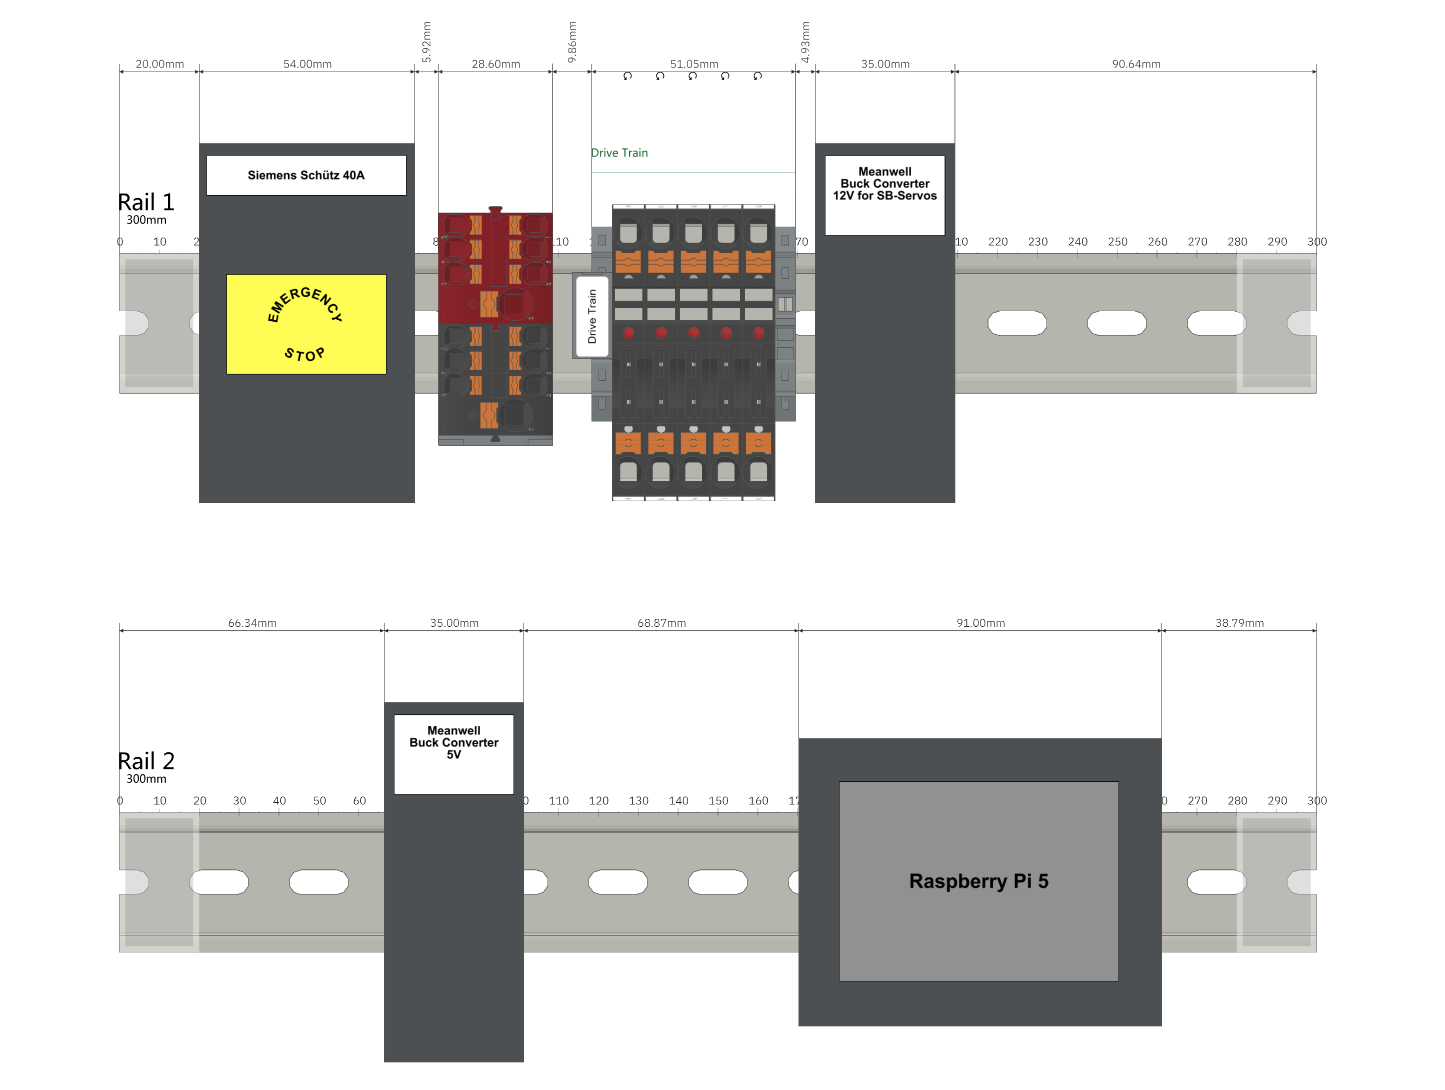
\includegraphics[width=1\linewidth]{contents/figures/bird-view_rails.png}
        \caption{Bird's-eye view onto the components. Several rails will be used stacked vertically in a wiring cabinet. The total length of rail can be calculated by summing up the width-units per rail and choosing a corresponding enclosure.}
        \label{bird-cad}
    \end{figure}

    \clearpage %PAGE SPECIFIER

    \begin{figure}[h!] %Float specifier check: passed!
        \vspace{1cm}
        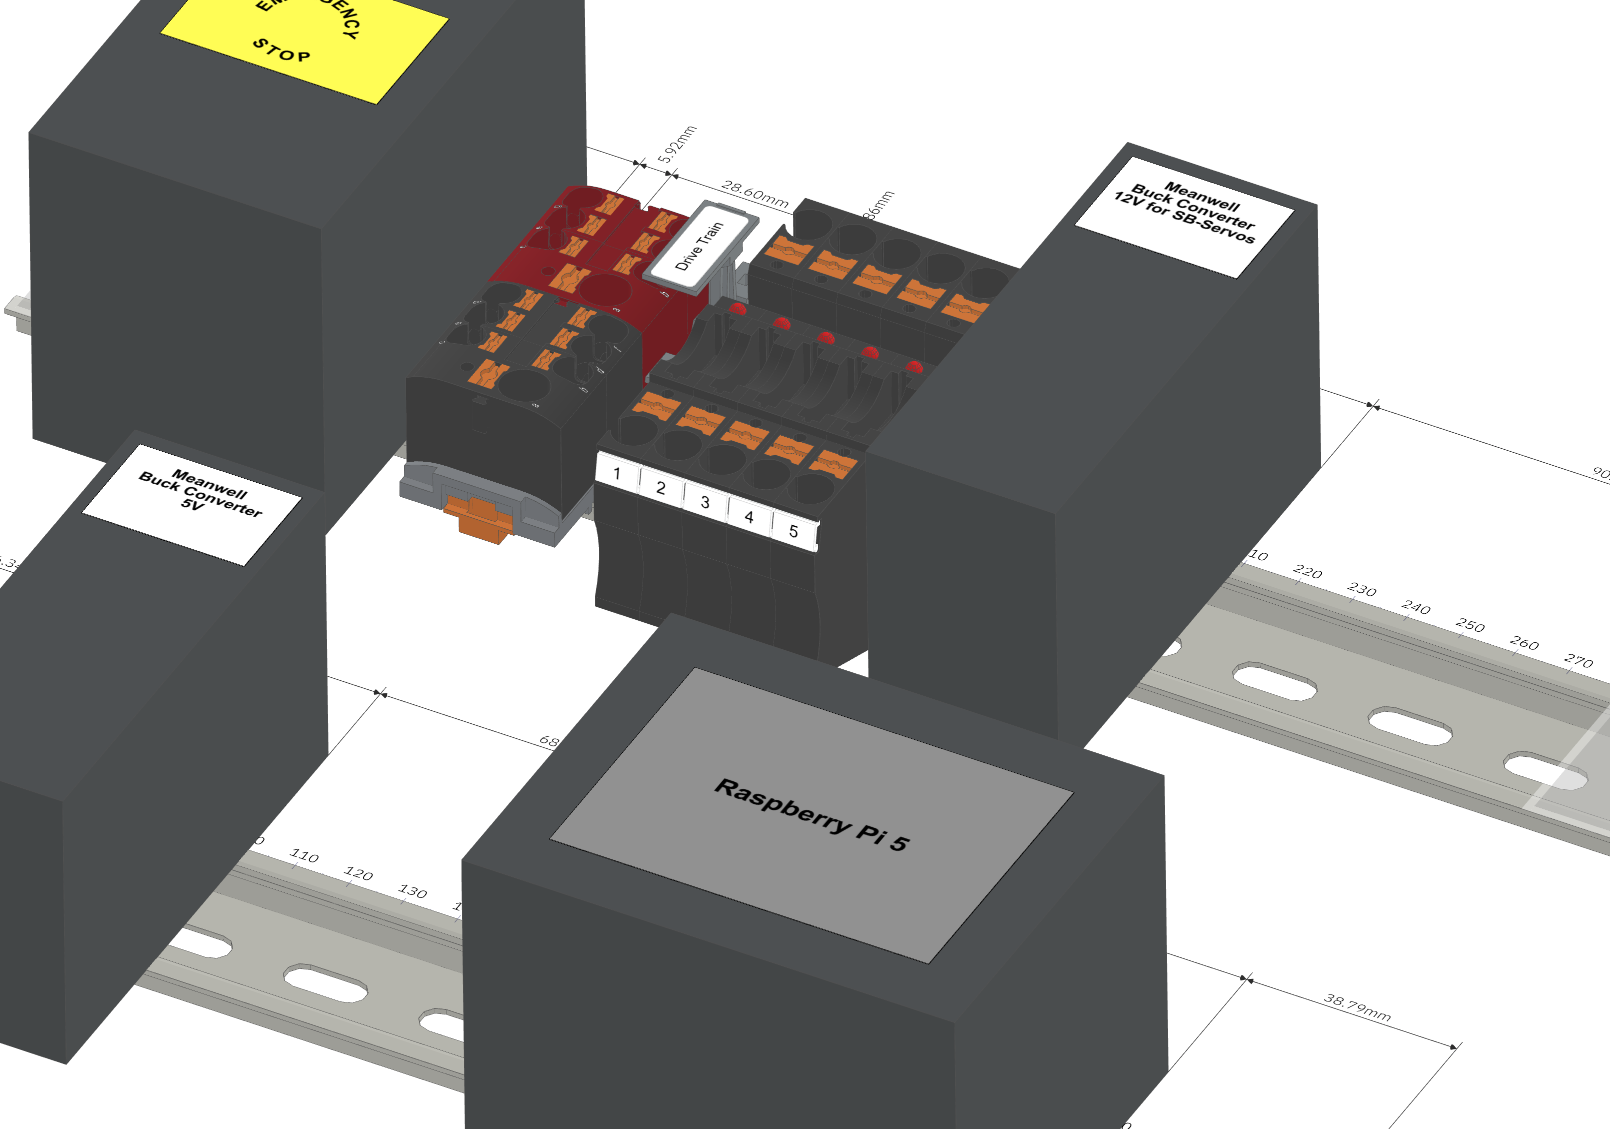
\includegraphics[width=1\linewidth]{contents/figures/diagonal-view_rails.png}
        \caption{3D mock-up of the components mounted onto DIN-rails. Also factors like the total height, heat dissipation, air flow and fans and must be taken into account. The majority of components are rendered as a "black box" to reduce overall complexity of the CAD design. Their exact surface can be modelled in the future, this is however not strictly necessary for general planning.}
        \label{diagonal-cad}
    \end{figure}

    

%\section{Energy Storage}

%\section{Emergency Stop}

%\section{Power Distribution}

%\section{Power Conversion}

%\section{Power Consuming Circuits}

%\section{Unused Circuits}

%\section{Circuit Table}

